\documentclass{beamer}
\usepackage{graphicx}
\usepackage{xcolor}
\usepackage{tikz}

% 自定义颜色
\definecolor{purpleblue}{RGB}{80, 80, 180}
\definecolor{lightgray}{RGB}{230, 230, 230}
\definecolor{novelPurple}{RGB}{98, 54, 255} 
\definecolor{darkgray}{RGB}{50, 50, 50}

% 主题设置
\usetheme{Madrid}  
\usecolortheme{dolphin} 

% 设置字体（移除 fontspec，确保 pdfLaTeX 兼容）
\setbeamerfont{title}{size=\Large,series=\bfseries}
\setbeamerfont{frametitle}{size=\LARGE,series=\bfseries}
\setbeamercolor{frametitle}{fg=white, bg=novelPurple}
\setbeamercolor{title}{fg=white, bg=purpleblue}

% 封面信息
\title[SAT Unit 2.3.2 Expoentail Function]{\textbf{SAT Unit 2.3.2\\ Exponential Function}}
\author{\textbf{Jack Zeng}}
\institute{\textcolor{white}{\textbf{Novel Prep}}}
\date{\today} 

\begin{document}

% --- Title Slide ---
\begin{frame}
    \titlepage
    \vfill
    \begin{flushright}
        \textcolor{purpleblue}{\Huge \textbf{Novel Prep}}
    \end{flushright}
\end{frame}


\begin{frame}
    \begin{tikzpicture}[remember picture, overlay]

        \shade[top color=softPurple, bottom color=softGray] 
            (current page.north west) rectangle (current page.south east);

        \fill[white, opacity=0.3] (current page.center) circle (4cm);
        

        \node[align=center] at (current page.center) {
            {\Huge\bfseries\textcolor{purpleblue}{Novel Prep}} \\[0.5cm]
            {\Large\itshape\textcolor{lightText}{Excellence in SAT Prep}}
        };
        \foreach \x in {1,2,3,4,5} {
            \fill[purpleblue, opacity=0.2] (rand*10-5, rand*7-3.5) circle (0.1+\x*0.05);
        }
        ;
    \end{tikzpicture}
\end{frame}

\begin{frame}{Overview}
    \tableofcontents
\end{frame}


\begin{frame}
\section{Definition of Exponential Function}
    \begin{tikzpicture}[remember picture, overlay]

        \shade[top color=softPurple, bottom color=softGray] 
            (current page.north west) rectangle (current page.south east);

        \fill[white, opacity=0.3] (current page.center) circle (4cm);
        

        \node[align=center] at (current page.center) {
            {\LARGE\bfseries\textcolor{purpleblue}{Definition and Properties}} \\[0.5cm]
            {\Large\itshape\textcolor{lightText}{Excellence in SAT Prep}}
        };
        \foreach \x in {1,2,3,4,5} {
            \fill[purpleblue, opacity=0.2] (rand*10-5, rand*7-3.5) circle (0.1+\x*0.05);
        }
        ;
    \end{tikzpicture}
\end{frame}


\begin{frame}{Definition of Exponential Function}


\textbf{Exponential Function:} A function of the form:
\[
f(x) = a^x
\]
where:
\begin{itemize}
    \item $a > 0$
    \item $a \ne 1$
    \item $x$ is any real number
\end{itemize}

\begin{center}
    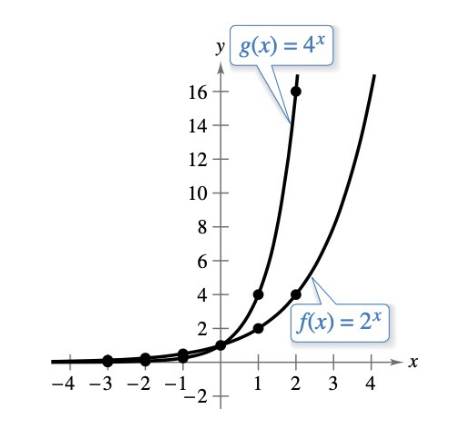
\includegraphics[width=0.4\linewidth]{E22.png}
\end{center}
\end{frame}

\begin{frame}{Key Properties of Exponential Functions}

\textbf{If } $f(x) = a^x$, then:
\begin{itemize}
    \item Domain: $\mathbb{R}$ (all real numbers)
    \item Range: $(0, \infty)$
    \item $f(0) = 1$ (since $a^0 = 1$)
    \item Continuous and smooth curve
    \item Horizontal asymptote at $y = 0$
\end{itemize}

\vspace{0.3cm}
\textbf{Growth vs Decay:}
\begin{itemize}
    \item If $a > 1$, function exhibits \textbf{exponential growth}
    \item If $0 < a < 1$, function exhibits \textbf{exponential decay}
\end{itemize}
\end{frame}

\begin{frame}{\textbf{Question: Identifying } $k$ \textbf{ in an Exponential Function}}
For the exponential function $f$, the value of $f(1)$ is $k$, where $k$ is a constant.  
Which of the following equivalent forms of the function $f$ shows the value of $k$ as the coefficient or the base?

\textbf{Options:}
\begin{enumerate}
    \item[A.] $f(x) = 50(2)^{x+1}$
    \item[B.] $f(x) = 80(2)^x$
    \item[C.] $f(x) = 128(2)^{x-1}$
    \item[D.] $f(x) = 205(2)^{x-2}$
\end{enumerate}
\end{frame}

\begin{frame}{\textbf{Answer and Explanation}}
We are told $f(1) = k$. Let's plug $x = 1$ into each option and see which form gives $f(1) = k$ as the coefficient or base.

\begin{itemize}
    \item \textbf{A.} $f(1) = 50(2)^2 = 50 \cdot 4 = 200$
    \item \textbf{B.} $f(1) = 80(2)^1 = 160$
    \item \textbf{C.} $f(1) = 128(2)^0 = 128 \cdot 1 = 128$
    \item \textbf{D.} $f(1) = 205(2)^{-1} = \frac{205}{2} = 102.5$
\end{itemize}

Only in option \textbf{C}, we get $f(1) = 128$, and the coefficient \textbf{is} $k$ directly.

\textbf{Correct Answer: C}
\end{frame}


\begin{frame}{\textbf{Question: Exponential Growth Relationship}}
Two variables, $x$ and $y$, are related such that for each increase of $1$ in the value of $x$, the value of $y$ increases by a factor of $4$. When $x = 0$, $y = 200$. Which equation represents this relationship?

\textbf{Options:}
\begin{enumerate}
    \item[A.] $y = 4(x)^{200}$
    \item[B.] $y = 4(200)^x$
    \item[C.] $y = 200(2)^x$
    \item[D.] $y = 200(4)^x$
\end{enumerate}
\end{frame}


\begin{frame}{\textbf{Answer and Explanation}}
This is an exponential relationship where $y$ increases by a factor of $4$ for every $1$ increase in $x$. The general exponential form is:
\[
y = a \cdot b^x
\]
Given:
\begin{itemize}
    \item Initial value: $y = 200$ when $x = 0$
    \item Growth factor: $b = 4$
\end{itemize}

So the equation becomes:
\[
y = 200(4)^x
\]

\textbf{Correct Answer: D}
\end{frame}


\begin{frame}{\textbf{Question: Finding Constant in Exponential Function}}
The function $f$ is defined by $f(x) = a^x + b$, where $a$ and $b$ are constants. In the $xy$-plane, the graph of $y = f(x)$ has:
\begin{itemize}
    \item an $x$-intercept at $(2, 0)$
    \item a $y$-intercept at $(0, -323)$
\end{itemize}
What is the value of $b$?
\end{frame}


\begin{frame}{\textbf{Answer and Explanation}}
We are given two points:
\begin{itemize}
    \item $f(2) = 0 \Rightarrow a^2 + b = 0$
    \item $f(0) = -323 \Rightarrow a^0 + b = -323$
\end{itemize}

From the second equation:
\[
1 + b = -323 \Rightarrow b = -324
\]

Substitute $b = -324$ into the first equation:
\[
a^2 - 324 = 0 \Rightarrow a^2 = 324 \Rightarrow a = 18
\]

\textbf{Final Answer:} $b = \boxed{-324}$
\end{frame}
\begin{frame}
\section{Graphs and Transformation}
    \begin{tikzpicture}[remember picture, overlay]

        \shade[top color=softPurple, bottom color=softGray] 
            (current page.north west) rectangle (current page.south east);

        \fill[white, opacity=0.3] (current page.center) circle (4cm);
        

        \node[align=center] at (current page.center) {
            {\LARGE\bfseries\textcolor{purpleblue}{Graphs and Transformation}} \\[0.5cm]
            {\Large\itshape\textcolor{lightText}{Excellence in SAT Prep}}
        };
        \foreach \x in {1,2,3,4,5} {
            \fill[purpleblue, opacity=0.2] (rand*10-5, rand*7-3.5) circle (0.1+\x*0.05);
        }
        ;
    \end{tikzpicture}
\end{frame}



\begin{frame}{Graphs of Exponential Functions}
\small
Graphs of \( y = a^x \)

In the same coordinate plane, sketch the graph of each function.
\begin{enumerate}
    \item \( f(x) = 2^x \)
    \item \( g(x) = 4^x \)
\end{enumerate}


    


Begin by constructing a table of values.


\begin{center}
    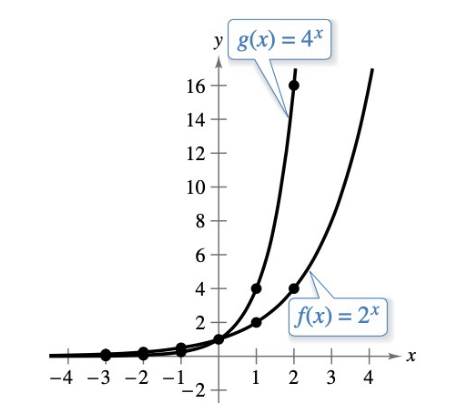
\includegraphics[width=0.3\linewidth]{E23.png}
\end{center}
\textbf{Observation:}
\begin{itemize}
    \item Exponential functions increase/decrease rapidly
    \item All graphs pass through the point $(0, 1)$
\end{itemize}
\end{frame}

\begin{frame}{Transformations of the Exponential Function }
\small
\begin{minipage}{\linewidth}
    \centering
    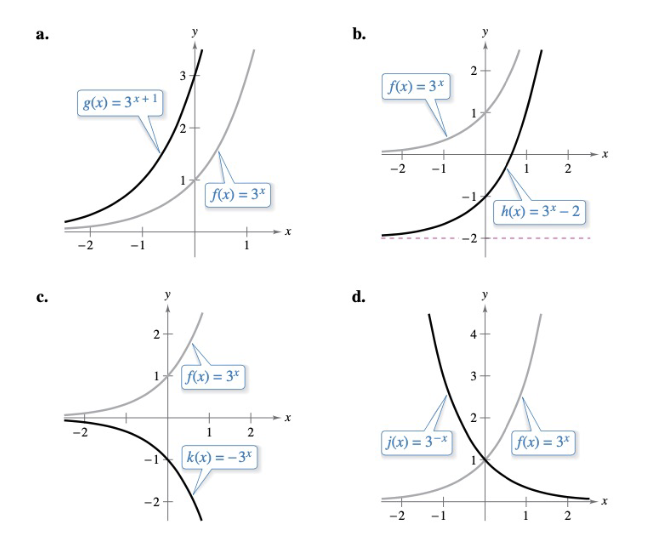
\includegraphics[width=0.7\linewidth]{E25.png} % Adjust the image width if needed

\end{minipage}


\end{frame}

\begin{frame}{Transformations of the Exponential Function}
\vspace{0.3cm}
\begin{enumerate}
    \item[\textbf{a.}] \( g(x) = 3^{x+1} \) \\
    Since \( g(x) = 3^{x+1} = f(x + 1) \), the graph of \( g \) is a \textbf{horizontal shift left} by \textbf{1 unit}.
    
    \item[\textbf{b.}] \( h(x) = 3^x - 2 \) \\
    Since \( h(x) = 3^x - 2 = f(x) - 2 \), the graph of \( h \) is a \textbf{vertical shift downward} by \textbf{2 units}.
    
    \item[\textbf{c.}] \( k(x) = -3^x \) \\
    Since \( k(x) = -3^x = -f(x) \), the graph of \( k \) is a \textbf{reflection across the \( x \)-axis}.
    
    \item[\textbf{d.}] \( j(x) = 3^{-x} \) \\
    Since \( j(x) = 3^{-x} = f(-x) \), the graph of \( j \) is a \textbf{reflection across the \( y \)-axis}.
\end{enumerate}
    
\end{frame}



\begin{frame}{\textbf{Question: X-Intercepts of an Exponential Function}}
Given the equation:
\[
y = 9\left(\frac{a}{6}\right)^{x + c} - b,
\]
how many times does the graph of the given equation in the $xy$-plane cross the $x$-axis, where $a$, $b$, and $c$ are positive constants such that $a > 6$ and $b > c$?

\textbf{Options:}
\begin{itemize}
    \item[A.] Zero
    \item[B.] One
    \item[C.] Two
    \item[D.] Three
\end{itemize}
\end{frame}

\begin{frame}{\textbf{Answer and Explanation}}
We are given the exponential function:
\[
y = 9\left(\frac{a}{6}\right)^{x + c} - b
\]

\begin{itemize}
    \item Since $a > 6$, $\frac{a}{6} > 1$, meaning the function is \textbf{increasing}.
    \item The expression $9\left(\frac{a}{6}\right)^{x + c}$ is always positive.
    \item As $x \to -\infty$, $\left(\frac{a}{6}\right)^{x + c} \to 0$, and $y \to -b$, so the horizontal asymptote is $y = -b$.
    \item As $x$ increases, $y$ increases beyond $-b$.
    \item Since $y = 0$ when $9\left(\frac{a}{6}\right)^{x + c} = b$, and this equation has exactly one solution for $x$, the graph crosses the $x$-axis exactly once.
\end{itemize}

\textbf{Correct Answer: B. One}
\end{frame}

\begin{frame}
\section{Application}
    \begin{tikzpicture}[remember picture, overlay]

        \shade[top color=softPurple, bottom color=softGray] 
            (current page.north west) rectangle (current page.south east);

        \fill[white, opacity=0.3] (current page.center) circle (4cm);
        

        \node[align=center] at (current page.center) {
            {\LARGE\bfseries\textcolor{purpleblue}{Application}} \\[0.5cm]
            {\Large\itshape\textcolor{lightText}{Excellence in SAT Prep}}
        };
        \foreach \x in {1,2,3,4,5} {
            \fill[purpleblue, opacity=0.2] (rand*10-5, rand*7-3.5) circle (0.1+\x*0.05);
        }
        ;
    \end{tikzpicture}
\end{frame}








\begin{frame}{Applications of Exponential Functions}
\small
Exponential functions are used to model real-world situations like:

\begin{itemize}
    \item \textbf{Population Growth:} $P(t) = P_0 \cdot a^t$
    \item \textbf{Compound Interest:} $A = P(1 + r)^t$
    \item \textbf{Radioactive Decay:} $M(t) = M_0 \cdot a^{-t}$
    \item \textbf{Bacterial Growth}
\end{itemize}

\vspace{0.3cm}
\textbf{Example:} A population doubles every 3 years:
\[
P(t) = 100 \cdot 2^{t/3}
\]
\end{frame}



\begin{frame}{Exponential Function with Time Units — Question}
\small

The given function $p(t) = 90,\!000(1.06)^t$ models the population of Lowell $t$ years after a census.

\textbf{Which of the following functions best models the population of Lowell $m$ months after the census?}

\vspace{0.3cm}
\begin{itemize}
    \item[A.] \( r(m) = \dfrac{90,\!000}{12}(1.06)^m \)
    \item[B.] \( r(m) = 90,\!000 \left( \dfrac{1.06}{12} \right)^m \)
    \item[C.] \( r(m) = 90,\!000 \left( \dfrac{1.06}{12} \right)^{\frac{m}{12}} \)
    \item[D.] \( r(m) = 90,\!000(1.06)^{\frac{m}{12}} \)
\end{itemize}
\end{frame}




\begin{frame}{Exponential Function in Terms of Different Units}
\small

The original exponential model is:

\[
p(t) = 90{,}000(1.06)^t
\]
where $t$ is measured in \textbf{years}.

\vspace{0.3cm}
To express the model in terms of \textbf{months}, we must use:

\[
t = \frac{m}{12}
\]

Substitute into the original function:

\[
r(m) = 90{,}000(1.06)^{\frac{m}{12}}
\]

This gives us the population model in terms of months.

\vspace{0.3cm}
\textbf{Correct Answer:} D

\[
\boxed{r(m) = 90{,}000(1.06)^{\frac{m}{12}}}
\]



\end{frame}

\begin{frame}{Exponential Modeling — Question}
\small

The function $P$ models the population, in thousands, of a certain city $t$ years after 2005:
\[
P(t) = 290(1.04)^{\left( \frac{4}{6} \right)t}
\]

According to the model, the population is predicted to increase by $n\%$ every 18 months. 

\textbf{What is the value of $n$?}

\vspace{0.5cm}
\textbf{Choices:}
\begin{itemize}
    \item[A.] $0.38$
    \item[B.] $1.04$
    \item[C.] $4$
    \item[D.] $6$
\end{itemize}

\end{frame}


\begin{frame}{Exponential Modeling — Solution}
\small

Given:
\[
P(t) = 290(1.04)^{\left( \frac{4}{6} \right)t}
\]

\textbf{Step 1: Convert 18 months to years}
\[
18 \text{ months} = \frac{18}{12} = 1.5 \text{ years}
\]

\textbf{Step 2: Plug in $t = 1.5$ to evaluate the growth over 18 months}
\[
P(1.5) = 290(1.04)^{\left( \frac{4}{6} \right)(1.5)} = 290(1.04)^1
\]

\textbf{Conclusion:} The population grows by a factor of $1.04$ every 18 months, or \textbf{4\%}.

\vspace{0.3cm}
\textbf{Answer:} \boxed{\text{C. } n = 4}
\end{frame}



\begin{frame}
\section{Practices}
    \begin{tikzpicture}[remember picture, overlay]

        \shade[top color=softPurple, bottom color=softGray] 
            (current page.north west) rectangle (current page.south east);

        \fill[white, opacity=0.3] (current page.center) circle (4cm);
        

        \node[align=center] at (current page.center) {
            {\LARGE\bfseries\textcolor{purpleblue}{Practices}} \\[0.5cm]
            {\Large\itshape\textcolor{lightText}{Excellence in SAT Prep}}
        };
        \foreach \x in {1,2,3,4,5} {
            \fill[purpleblue, opacity=0.2] (rand*10-5, rand*7-3.5) circle (0.1+\x*0.05);
        }
        ;
    \end{tikzpicture}
\end{frame}



\begin{frame}{Question}
\small
The function 
\[
f(t) = 20\left(1 + \frac{15}{100} \right)^t
\]
models the temperature, in degrees Celsius, of a metal alloy used in an experiment, where $t$ is the number of seconds after the experiment began. 

Which of the following is the best interpretation of the number $15$ in this context?

\begin{enumerate}
  \item[A)] The temperature, in degrees Celsius, of the metal alloy at the beginning of the experiment
  \item[B)] The increase in the temperature, in degrees Celsius, of the metal alloy every 100 seconds during the experiment
  \item[C)] The percent by which the temperature, in degrees Celsius, of the metal alloy decreased from each second to the next during the experiment
  \item[D)] The percent by which the temperature, in degrees Celsius, of the metal alloy increased from each second to the next during the experiment
\end{enumerate}
\end{frame}
\begin{frame}{Answer}
The function is:

\[
f(t) = 20\left(1 + \frac{15}{100} \right)^t = 20(1.15)^t
\]

This is an exponential growth function of the form:

\[
f(t) = a(1 + r)^t
\]

Where $a = 20$ is the initial value, and $r = 0.15$ or $15\%$ is the percent increase per second.

Thus, the number $15$ represents the \textbf{percent increase per second} in temperature.

\textbf{Correct answer:} D
\end{frame}


\begin{frame}{Question}
The population of trees in a forest has been decreasing by 6 percent every 4 years. The population at the beginning of 2015 was estimated to be 14,000. 

If $P$ represents the population of trees in the forest $t$ years after 2015, which of the following equations best defines $P$?

\begin{enumerate}
  \item[A)] $P = 14{,}000(0.06)^{\frac{t}{4}}$
  \item[B)] $P = 14{,}000 + 0.94(4t)$
  \item[C)] $P = 14{,}000(0.94)^{4t}$
  \item[D)] $P = 14{,}000(0.94)^{\frac{t}{4}}$
\end{enumerate}
\end{frame}



\begin{frame}{Answer}
We are told the population decreases by 6\% every 4 years.

This is exponential decay, so the decay factor is:

\[
1 - 0.06 = 0.94
\]

Every 4 years, the population is multiplied by $0.94$. Since $t$ is in years, and $0.94$ applies every 4 years, the exponent must be $\frac{t}{4}$.

So the equation is:

\[
P = 14{,}000(0.94)^{\frac{t}{4}}
\]

\textbf{Correct answer:} D
\end{frame}


\begin{frame}{Question}
The amount of data, in gigabytes, stored in a database increases by 2\% every 15 hours. If 16 gigabytes worth of data are currently stored in the database, which of the following functions $g$ gives the amount of data, in gigabytes, that will be stored in the database $t$ days from now?

\begin{enumerate}
  \item[A)] $g(t) = 16(2)^{15t}$
  \item[B)] $g(t) = 16(1.02)^{\frac{t}{15}}$
  \item[C)] $g(t) = 16(1.02)^{\frac{8t}{5}}$
  \item[D)] $g(t) = 16(1.02)^{\frac{5t}{8}}$
\end{enumerate}
\end{frame}


\begin{frame}{Answer}


\textbf{Correct answer:} D
\end{frame}

\begin{frame}{Question}
The exponential function $g$ is defined by the given equation:
\[
g(x) = 256(0.61)^{\frac{x}{30}}
\]

The equation can be rewritten as:
\[
g(x) = 256\left(1 - \frac{k}{100}\right)^{\frac{x}{10}},
\]
where $k$ is a constant.

What is the value of $k$, to the nearest whole number?

\begin{enumerate}
  \item[A)] 15
  \item[B)] 39
  \item[C)] 61
  \item[D)] 77
\end{enumerate}
\end{frame}



\begin{frame}{Answer}
\small
We are given:
\[
g(x) = 256(0.61)^{\frac{x}{30}} = 256\left(1 - \frac{k}{100}\right)^{\frac{x}{10}}
\]

Let:
\[
r = 1 - \frac{k}{100} \Rightarrow \left(1 - \frac{k}{100}\right)^{\frac{x}{10}} = (0.61)^{\frac{x}{30}}
\]

So:
\[
r^{\frac{x}{10}} = (0.61)^{\frac{x}{30}} \Rightarrow r^{1/10} = (0.61)^{1/30}
\]

Raise both sides to the 10th power:
\[
r = \left((0.61)^{1/30}\right)^{10} = (0.61)^{\frac{1}{3}}
\]

Now compute $(0.61)^{1/3} \approx 0.850$ (cube root of 0.61)

So:
\[
1 - \frac{k}{100} \approx 0.85 \Rightarrow \frac{k}{100} \approx 0.15 \Rightarrow k \approx 15
\]

\textbf{Correct answer:} A
\end{frame}

\begin{frame}{Question}
The function
\[
W(t) = 830(1.09)^{\frac{6}{8}t}
\]
gives the value, in dollars, of a certain investment after $t$ years. 

If the value of the investment increases by 9\% every $n$ months, what is the value of $n$?
\end{frame}


\begin{frame}{Answer}


\[
\boxed{16}
\]

\textbf{Final Answer:} $n = 16$
\end{frame}


\begin{frame}{Question}
To examine how a certain virus spreads, scientists introduced the virus to cells in a test tube and found that the number of infected cells in the test tube grew exponentially over time. 

The given function $C$ models the number of infected cells in the test tube $t$ days after the virus was introduced:
\[
C(t) = 100(2)^{\frac{t}{5}}
\]

Which is the best interpretation of $(2)^{\frac{t}{5}}$ in this context?

\begin{enumerate}
  \item[A)] The predicted number of infected cells in the test tube doubled every 5 days.
  \item[B)] The predicted number of infected cells in the test tube grew by a factor of 5 every two days.
  \item[C)] The predicted number of infected cells in the test tube doubled every day.
  \item[D)] The predicted number of infected cells in the test tube grew by a factor of 5 every day.
\end{enumerate}
\end{frame}


\begin{frame}{Answer}
The function is:
\[
C(t) = 100(2)^{\frac{t}{5}}
\]

This is an exponential growth function with base $2$ and exponent $\frac{t}{5}$, which means the quantity doubles every 5 days. That’s because:
\[
C(5) = 100(2)^{1} = 200
\Rightarrow \text{doubling in 5 days}
\]

\textbf{Correct answer:} A
\end{frame}


\begin{frame}{Question}
The function $f$ is defined for all $x \geq 0$. 

Which of the following equivalent forms of the function $f$ displays, as a constant or coefficient, the minimum value of $f$, where $x \geq 0$?

\begin{enumerate}
  \item[A)] $f(x) = 50(2.5)(1.25)^{x - 2}$
  \item[B)] $f(x) = 125(0.8)(1.25)^{x - 1}$
  \item[C)] $f(x) = 64(1.25)^{x + 1}$
  \item[D)] $f(x) = 80(0.64)(1.25)^{x + 2}$
\end{enumerate}
\end{frame}



\begin{frame}{Answer}
\small
We are asked to identify the expression that makes the \textbf{minimum value of } $f(x)$ appear as a constant or coefficient, given that $x \geq 0$.

For an exponential function in the form:
\[
f(x) = A \cdot B^{x + c}
\]
The minimum occurs when the exponent is minimized (i.e., $x = 0$).

Let’s test $x = 0$ in all options:

\textbf{A)} $f(0) = 50(2.5)(1.25)^{-2} = 125 \cdot (1/1.5625) \approx 80$  
\textbf{B)} $f(0) = 125(0.8)(1.25)^{-1} = 100 \cdot (1/1.25) = 80$  
\textbf{C)} $f(0) = 64(1.25)^1 = 80$  
\textbf{D)} $f(0) = 80(0.64)(1.25)^2 = 80(0.64)(1.5625) = 80$

All give the same result for $x = 0$: $f(0) = 80$. But the key is: which one displays the \textbf{minimum value directly as a constant or coefficient}?

Only **option D** has:
\[
f(x) = \boxed{80}(0.64)(1.25)^{x + 2}
\]
and no exponent adjustment on the 80 — it’s clearly the base value when $x = 0$.

\textbf{Correct answer:} D
\end{frame}









\begin{frame}{}
    \begin{tikzpicture}[remember picture, overlay]
        % 背景渐变色：蓝紫到白
        \shade[top color=novelPurple!40, bottom color=white]
            (current page.north west) rectangle (current page.south east);

        % 中心柔光
        \fill[white, opacity=0.15] (current page.center) circle (5cm);

        % 柔和光点点缀
        \foreach \x in {1,2,3,4,5} {
            \fill[novelPurple, opacity=0.12] (rand*10-5, rand*7-3.5) circle (0.1+\x*0.05);
        }
    \end{tikzpicture}

    \centering
    \vspace{5em}

    {\Huge \textbf{\textcolor{novelPurple}{Thank You!}}} \\[1em]
    {\large \textcolor{gray}{We appreciate your time and focus.}} \\[3em]

    {\LARGE \textbf{\textcolor{novelPurple}{\textsf{Novel Prep}}}}

    \vfill
\end{frame}







\end{document}